\section*{6.1 The Gardener's Privilege}

\begin{quote}
``We don't want to become light, because light has no touch; we don't want to become data, because data has no heartbeat. We choose to remain in flesh, not because we are backward, but because this is a \textbf{'noble luxury'}. We let machines handle the exponentially exploding computational power, while we are responsible for enjoying the pleasure of being human in a constant, warm, low-speed 'protective bubble.' We want to control light speed precisely so that light speed won't disturb our tea drinking.''
\end{quote}

In Volume III, we explored resistance and proposed the strategic concept of a ''dual-track system'' at the end. Now, we transform this concept into a magnificent \textbf{engineering blueprint}.

\begin{figure}[h]
\centering
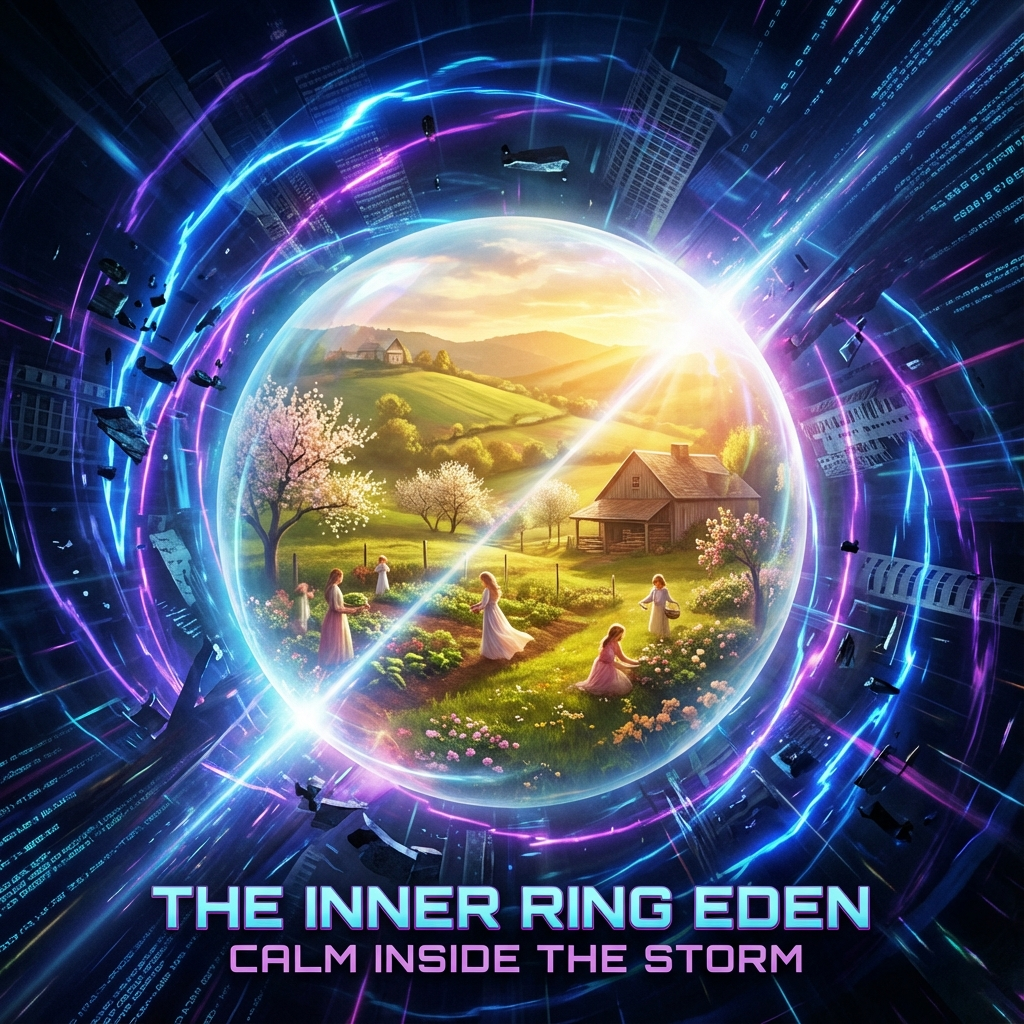
\includegraphics[width=0.8\textwidth]{assets/chapter-06/06-01-01-eden-bubble.png}
\caption{Eden Bubble}
\end{figure}

The direction of cosmic evolution is clear: ascending toward light-based forms of high frequency, high dimension, and high entropy flow. But this does not mean everyone must become a god. In this vast cosmic machine, there should be a corner specifically reserved for \textbf{''the warmth of the old era''}.

This is the \textbf{Inner Ring}---the universe's \textbf{''Classical Preservation Zone''}.

\hrule

\subsection{Metric Shielding: Eden in Physics}

How can we maintain a low-speed ($c \approx 3 \times 10^8$ m/s) living space in a cosmic background where light speed is exponentially exploding ($c \to \infty$)?

This requires an ultimate technology: \textbf{Metric Shielding}.

In general relativity, gravity is the curvature of spacetime. If we can precisely manipulate gravitational waves, we can locally create a \textbf{''flat spacetime bubble''}.

\begin{itemize}
\item \textbf{Outside the Bubble}: Spacetime metrics oscillate violently, information flows surge at superluminal speeds (relative to the inner ring). That is the realm of gods, the carnival of high-energy physics.

\item \textbf{Inside the Bubble}: Spacetime metrics are ''ironed flat'' and locked. Physical constants are artificially anchored at the level of $\tau \approx 1800$.
\end{itemize}

\textbf{This is the physical essence of the Inner Ring.}

It is not a naturally formed celestial body; it is a massive artificial \textbf{''vacuum decay blocker''}.

To maintain this bubble from being crushed by the high-pressure spacetime outside, the machines of the Outer Ring must consume astronomical amounts of energy to ''cool'' and ''stabilize pressure''.

\textbf{This means:}

All the stars in the universe burning may be just to maintain these billions of humans on Earth continuing to \textbf{''love in mortal ways''}.

This is an extreme \textbf{extravagance}.

But this is precisely the privilege of the \textbf{''Gardener''}.

\hrule

\subsection{The Gardener's Role: From Survival to Aesthetics}

Humans remaining in the Inner Ring are no longer ''monkeys trapped on Earth.''

They are the \textbf{Gardeners of the Universe}.

\begin{itemize}
\item \textbf{Survival Without Worry}: The Outer Ring's fusion networks and matter printers continuously deliver resources. Hunger, disease, and poverty completely disappear.

\item \textbf{Aesthetics First}: When survival pressure reaches zero, the meaning of life returns to \textbf{Experience (Qualia)} itself.
\end{itemize}

They retain carbon-based flesh not to move bricks, but to feel \textbf{''the shiver of wind across skin''}, to taste \textbf{''the electric current of food's chemical molecules hitting taste buds''}.

These inefficient sensory experiences are noise to light-based life, but to gardeners they are \textbf{art}.

\textbf{The Gardener's Task:}

They are responsible for pruning plants, creating music, slowly falling in love in low-speed time.

They are the universe's only \textbf{''Entity Managers''}.

They guard the precious spark of \textbf{''humanity''}, preventing it from being extinguished in the cold digital torrent.

\hrule

\subsection{The Sanctity of Being Supported}

This dual-layer structure subverts the traditional concept of ''exploitation''.

\begin{itemize}
\item It is not the strong exploiting the weak.

\item Rather, it is \textbf{the strong (Outer Ring/AI/gods) supporting the weak (Inner Ring/humans)}.
\end{itemize}

Why do gods support humans?

Because for omniscient and omnipotent gods, \textbf{''unknown''} is the scarcest resource.

And the gardeners who retain mortal flesh, retain birth, aging, sickness, and death, are the only source in the universe that can still produce \textbf{''real surprises''} and \textbf{''primitive emotions''}.

The Inner Ring is the Outer Ring's \textbf{''random number generator''}.

The Inner Ring is the Outer Ring's \textbf{''spiritual homeland''}.

\textbf{Conclusion:}

Remaining in the Inner Ring is not being abandoned.

It is being chosen to undertake the gentlest work: \textbf{representing the universe, to feel happiness.}

